\section*{3. Análisis de aplicaciones similares}

Para contextualizar el desarrollo de la plataforma propuesta, resulta imprescindible realizar un 
estudio del estado del arte que identifique las soluciones actuales, sus fortalezas y sus carencias
 tecnológicas. En este apartado se lleva a cabo un análisis comparativo de las herramientas más 
 representativas del ecosistema \textit{Fantasy} en España, evaluando tanto plataformas comerciales
  consolidadas como proyectos de código abierto.
  
  El objetivo de este examen es definir un marco de
   referencia funcional, detectar oportunidades de innovación y justificar las decisiones de diseño que 
   permitirán dotar a este proyecto de un valor añadido diferencial. El estudio comienza con el análisis
    de AnalíticaFantasy.com, uno de los referentes actuales en la gestión de datos estadísticos aplicados
     al juego.

\subsection{3.1 AnalíticaFantasy.com}

\subsubsection{3.1.1 Descripción general de la plataforma}

La web analizada proporciona un entorno completo para el seguimiento del fútbol y el 
Fantasy Football. En su página principal, la aplicación muestra noticias destacadas y un componente 
de actualización en tiempo real sobre el estado de forma de los jugadores, indicando cambios 
relevantes como ``duda leve'' a ``disponible''. Además, ofrece información sobre los partidos de las 
próximas dos jornadas, mostrando la alineación probable de cada equipo y estimaciones de titularidad 
para los jugadores. La plataforma también proporciona informes comparativos sobre goles, partidos 
jugados, penaltis, tarjetas y otras métricas, así como indicadores de la probabilidad de que cada 
equipo gane, ofreciendo así una visión integral del rendimiento y contexto competitivo.

\subsubsection{3.1.2 Detalles de equipos}

En la vista de cada equipo, se ofrece información completa sobre el próximo partido, 
incluyendo el rival y el horario del encuentro, así como la alineación probable con estimaciones de 
titularidad para cada jugador. Además, incorpora información contextual como las condiciones 
meteorológicas durante el partido, el registro de encuentros recientes del equipo y estadísticas de 
la temporada, incluyendo partidos jugados, ganados, empatados, perdidos, goles a favor y en contra, 
y las formaciones empleadas.

La plataforma también integra noticias relacionadas con el equipo y una sección interactiva de 
encuestas en la que los usuarios pueden votar sobre qué equipo creen que ganará el próximo partido. 
La información Fantasy del equipo se complementa mostrando los jugadores con más puntos totales, 
mejor media, mayor valor de mercado y aquellos que han incrementado su precio recientemente. 
Asimismo, se incluyen detalles sobre jugadores lesionados, sancionados o apercibidos, y estadísticas 
puramente deportivas, como minutos jugados, goles, asistencias, suplencias y titularidades.

Además, debajo de la zona de suplentes incluye un componente que a cada posición asigna una 
dificultad, pero en ningún momento se detalla en base a qué se toma esa decisión.
\begin{figure}[H]
\centering
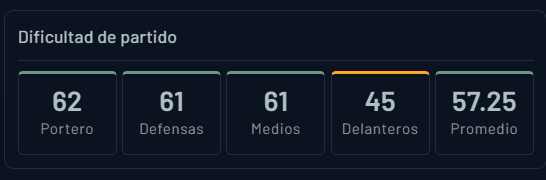
\includegraphics[width=0.58\textwidth]{images/similares1.png}
\caption{Figura de referencia de la dificultad de un partido en AnalíticaFantasy.com.}\label{fig:analitica-equipo}
\end{figure}

\subsubsection{3.1.3 Análisis detallado de partidos}

La aplicación permite la visualización de partidos pasados con un alto nivel de detalle. Para cada 
encuentro, se muestran el resultado final, los goleadores, las tarjetas recibidas y los minutos 
jugados por cada jugador. Sobre las alineaciones se representan gráficamente los puntos obtenidos en 
cada modelo Fantasy, pudiendo cambiar la referencia mediante botones interactivos.

Al hacer clic sobre un jugador, se despliega un modal con toda la información individual. La 
plataforma también muestra los resultados de las encuestas relacionadas con el partido y gráficas 
que resumen estadísticas del equipo, incluyendo partidos jugados, ganados, empatados, perdidos, 
goles a favor y en contra y puntos obtenidos. Además, se registra cronológicamente cada suceso del 
encuentro, como cambios, goles y tarjetas, proporcionando un análisis completo y visual de todos los 
eventos significativos.

De nuevo en esta vista se incluye información sobre los partidos pasados y próximos de cada equipo.

\subsubsection{3.1.4 Apartado H2H}

La aplicación incluye un módulo denominado ``H2H'' que permite analizar enfrentamientos previos entre 
dos equipos, incorporando datos históricos de varias temporadas. Este apartado facilita la 
comparación directa de resultados y tendencias de rendimiento entre rivales específicos, apoyando el 
análisis predictivo y estratégico dentro del Fantasy Football.

\subsubsection{3.1.5 Detalles de jugadores}

Cada jugador dispone de una vista individual en la que se presenta información personal, equipo y 
posición, junto con los puntos esperados en la próxima jornada diferenciando si con una estimación 
diferente en función de si es titular o no. Se incluyen la media de puntos obtenidos en casa y 
fuera, el valor actual del jugador, así como su valor máximo y mínimo y la estimación de puja ideal 
dentro del Fantasy.

La plataforma también ofrece un histórico de los partidos de la temporada, puntos obtenidos y la 
información sobre las posiciones en las que ha jugado, permitiendo un análisis completo del 
rendimiento y evolución del jugador.

Además del perfil se puede navegar a otros apartados, como ``Puntos'', donde se clasifica cada 
partidos del jugador en un rango según los puntos obtenidos, acompañado de un histograma, con el eje 
X siendo los partidos y el Y los puntos obtenidos. De forma similar, hay apartados de \textit{Minutos}, 
\textit{Mercado}, \textit{Calendario} y \textit{Proyección}, mostrando diferentes datos y gráficas del jugador y su 
valor de mercado.

\subsubsection{3.1.6 Seguimiento de jugadores}

La aplicación incorpora un apartado específico para el seguimiento de ``Jugadores'', en la barra 
lateral, que se identifican los jugadores lesionados junto con el tipo de lesión y el tiempo 
estimado de recuperación. También se muestran los jugadores sancionados, indicando el motivo y la 
duración de la sanción, así como los jugadores apercibidos de sanción, lo que permite a los usuarios 
anticipar riesgos y gestionar su equipo Fantasy de manera más estratégica.

\subsubsection{3.1.7 Predicciones}

Desde el menú lateral también se puede navegar hacia ``Predicciones Fantasy'', contrariamente a lo 
que parece, esta vista tan solo permite al usuario tratar de predecir resultados de partidos futuros 
y jugadores que destacarán, positiva y negativamente.

\subsubsection{3.1.8 Gestión de plantilla}

Incorpora una vista donde el usuario puede configurar su equipo sobreimpresionado en un campo de 
fútbol, pudiendo elegir entre diferentes formaciones y todos los jugadores de la liga. Para cada 
jugador se muestra el próximo partido, la probabilidad de ser titular y el valor de mercado.

Adicionalmente ofrece información una vez se ha confeccionado la plantilla, muestra datos agregados 
de goles, puntos, asistencias y otros factores determinantes.

\subsection{3.2 JornadaPerfecta.com}

\subsubsection{3.2.1 Descripción general de la plataforma}

La aplicación web analizada ofrece un acceso integral a la información de LaLiga y su ecosistema 
Fantasy. En la página de inicio, los usuarios pueden visualizar todos los equipos de la liga y 
acceder a sus detalles individuales, así como consultar un listado completo de los partidos de la 
próxima jornada para acceder a sus respectivos informes. Gran parte de la página principal se dedica 
a noticias destacadas y promociones de la aplicación, incluyendo gran cantidad publicidad de casas de 
apuestas, cuya visualización requiere desactivar bloqueadores de anuncios.

\subsubsection{3.2.2 Próximos partidos}

En la vista de próximos partidos, la plataforma presenta información detallada sobre fecha y hora de 
los encuentros, alineaciones probables y datos visuales que reflejan la participación de los 
jugadores en los últimos tres partidos mediante indicadores de color (rojo, naranja o verde) para 
titular o suplente. Además, se alerta sobre jugadores apercibidos de sanción.

Se incluye además, información sobre los próximos partidos de cada uno de los equipos y detalles de 
la retransmisión deportiva.

Esta sección mantiene la presencia de noticias y publicidad, integrando la información de manera 
visualmente destacada para los usuarios.
\begin{figure}[H]
\centering
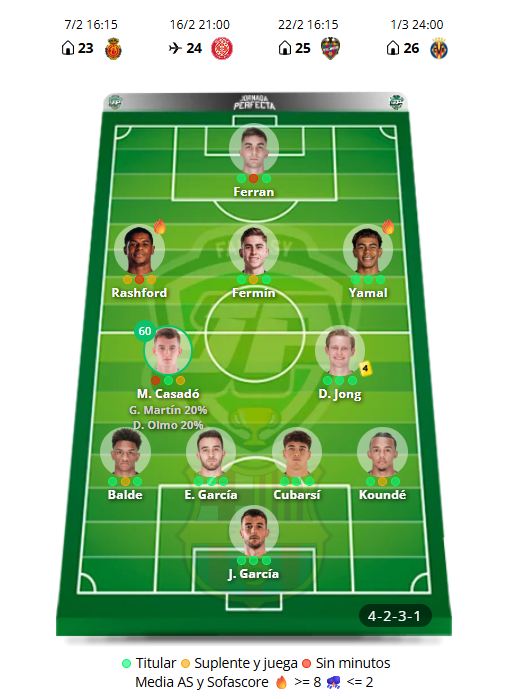
\includegraphics[width=0.58\textwidth]{images/similares2.png}
\caption{Figura de referencia de la vista de la plantilla de un equipo en JornadaPerfecta.com.}\label{fig:jornada-proximos-partidos}
\end{figure}

\subsubsection{3.2.3 Detalles de equipo}

La vista de cada equipo proporciona la alineación probable con elementos visuales adicionales que 
destacan información relevante de cada jugador. La plataforma incluye datos sobre jugadores no 
disponibles por sanción o lesión, así información especialmente relevante como los lanzadores 
habituales de faltas, penaltis y córners.

Además, se presentan actuaciones recientes de los jugadores, incluyendo los puntos obtenidos en los 
partidos y su posición, así como el valor de mercado dentro de la aplicación de Biwenger.

\subsubsection{3.2.4 Noticias y recomendaciones}

El apartado de noticias combina información deportiva con recomendaciones de fichajes o traspasos, 
presentadas de manera visualmente clara y destacada. Esta sección también incluye un espacio de 
comentarios utilizado por los usuarios para compartir dudas o solicitar consejos sobre decisiones a 
tomar en sus equipos Fantasy, fomentando la interacción y el intercambio de información entre la 
comunidad.
\begin{figure}[H]
\centering
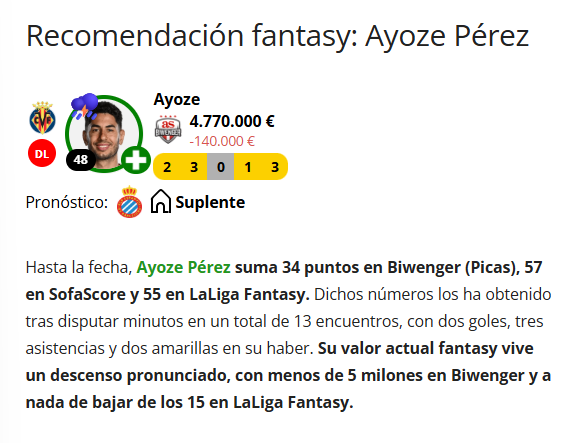
\includegraphics[width=0.58\textwidth]{images/similares3.png}
\caption{Figura de referencia del apartado de noticias.}\label{fig:jornada-noticias-recomendaciones}
\end{figure}

\subsubsection{3.2.5 Mercado}

Se incluye un apartado donde el usuario puede ver el valor de mercado de cada jugador, 
cuenta con diferentes filtros donde se puede elegir entre otros: modelo de puntuación fantasy, equipo, 
posiciones\ldots Adicionalmente muestra el listado de jugadores con información histórica del precio de 
cada jugador.

\subsubsection{3.2.6 Seguimiento de jugadores lesionados}

La plataforma incorpora una vista específica dedicada a los jugadores lesionados, organizada por 
equipos, que muestra información detallada sobre la lesión de cada jugador y el plazo estimado de 
regreso a la competición. Este apartado permite a los usuarios gestionar sus plantillas considerando 
las bajas y planificando estrategias alternativas de manera más informada.

\subsubsection{3.2.7 Detalles de jugador}

La vista individual de cada jugador ofrece información básica sobre su participación en los partidos 
recientes. Se muestran su posición, dorsal y valor de mercado tanto en Biwenger como en LaLiga 
Fantasy. La plataforma incluye un registro histórico de puntos de cada jornada, diferenciando entre 
partidos disputados en casa y fuera, y presenta información sobre los próximos encuentros del 
jugador. Complementariamente, se incorpora un gráfico que representa la evolución del valor de 
mercado del jugador durante el último mes en ambos mercados, acompañado nuevamente de noticias y 
actualizaciones relevantes sobre su rendimiento y situación deportiva.

\subsection{3.3 Repositorios}

\subsubsection{3.3.1 Repositorios analizados}

Se han explorado proyectos como ``Football-Prediction'' y ``LaLiga-Prediction-Analytics'', los 
cuales han permitido comprender el flujo de trabajo típico en este tipo de proyectos y las 
tecnologías que suelen utilizarse, como pandas, scikit-learn y Matplotlib. Además, estos proyectos 
han servido para evaluar si las fuentes de información planteadas inicialmente, FBref.com y 
futbolfantasy.com, son realmente fiables. Se comprobó que, en su mayoría, se utiliza FBref como 
fuente principal, lo que confirma la intuición inicial de que se trata de un sitio con datos 
confiables.

La principal diferencia y limitación respecto al proyecto que se va a realizar radica en el nivel de 
predicción. Mientras que estos repositorios se centran en predecir el resultado final de una 
temporada o los resultados de un partido con cierta probabilidad, por ejemplo:

\begin{figure}[H]
\centering
\fbox{%
\begin{minipage}{0.82\textwidth}
\small
Home: Barcelona \textbar\ Away: Real Madrid\\
Predicted: Home Win \textbar\ Confidence: 78\%
\end{minipage}%
}
\caption{Salida de la API de predicción mencionada en el análisis.}
\end{figure}

no ofrecen información detallada a nivel de jugadores.

En el presente proyecto, será necesario realizar scraping de información más detallada, no solo de 
los partidos en sí, sino de los jugadores que participan en cada partido. Esto añade una capa de 
complejidad significativa, ya que la obtención de los datos será más extensa y requerirá un mayor 
preprocesamiento para unificar y limpiar la información.

\subsubsection{3.3.2 Repositorios sin mantenimiento}

Se han encontrado otros repositorios, entre ellos ``laliga-fantasy-bot'', 
``marca-fantasy-api-scraper-updated'' y ``laligafantasy'', en busca de proyectos con 
características similares al presente trabajo. La mayoría de estos proyectos funcionan únicamente 
como scrapers, limitándose a generar un archivo.csv con información de jugadores que varía según el 
repositorio consultado (minutos jugados, valor de mercado, etc.).

El repositorio más parecido fue ``laligafantasy'', que ofrecía recomendaciones de alineaciones 
consideradas óptimas según la suma de puntos estimada y sugería al usuario incluso la formación a 
utilizar. Otras funcionalidades del proyecto no pudieron ser verificadas debido a la falta de 
mantenimiento, lo que constituye la principal limitación al buscar repositorios de código similares.

Todos estos proyectos tienen entre 2 y 6 años de antigüedad, carecen de mantenimiento y presentan 
numerosas issues abiertas, muchas de las cuales indican que ya no funcionan correctamente.

Durante este análisis también se identificó una limitación importante para el desarrollo del presente 
trabajo: ya no existe una API pública de LaLiga Fantasy. Todos sus endpoints han sido migrados a 
Android, lo que hace imposible realizar scraping para obtener información actualizada sobre el valor 
de mercado de los jugadores. Aunque se podría trabajar con datos de la temporada actual, se decidió 
omitir la gestión del mercado para mantener coherencia con los datos históricos utilizados en el 
entrenamiento del modelo.

\subsection{3.4 Conclusiones y valor añadido}

El análisis detallado de plataformas como FutbolFantasy.com y AnalíticaFantasy.com, junto con los repositorios relacionados, se ha encontrado un conjunto de 
funcionalidades recurrentes. Todas estas soluciones proporcionan un análisis exhaustivo de los 
encuentros disputados, incluyendo resultado final, goleadores, alineaciones titulares y suplentes, 
puntuaciones Fantasy por jugador, minutos jugados y eventos relevantes como tarjetas y cambios, así 
como estadísticas generales del partido (tiros, córners, pases, etc.).

Cada web integra vistas detalladas de jugadores con información esencial: posición y dorsal, 
valor de mercado actual, histórico de puntuaciones por jornada, comparativas de rendimiento en casa 
versus fuera, y estado del jugador (disponible, lesionado o sancionado). Asimismo, todas implementan 
un seguimiento completo de la disponibilidad de jugadores, incluyendo lesiones con tiempo estimado de 
recuperación, sanciones y jugadores apercibidos de riesgo de sanción próxima.

A nivel de equipo, las plataformas ofrecen datos consolidados como clasificación, próximos partidos, 
calendario completo, alineación probable y estadísticas de temporada (partidos jugados, ganados, 
empatados, perdidos, goles a favor y en contra). También incorporan información de los mercados 
Fantasy más populares, mostrando valor de mercado, estimaciones de titularidad y cambios recientes de 
precio. Finalmente, se incluyen datos contextuales como noticias, comparativas H2H y condiciones del 
partido (horario, lugar y clima).

\subsubsection{3.4.1 Limitaciones identificadas del presente trabajo}

Uno de los principales obstáculos técnicos radica en la inaccesibilidad de datos financieros en tiempo 
real. Debido a que, como se ha comentado, la API pública de LaLiga Fantasy ha restringido sus 
endpoints y los ha migrado a entornos cerrados de aplicaciones móviles, resulta imposible realizar un 
scraping automatizado y estable para obtener los valores de mercado de los jugadores. Esta carencia 
de una fuente de datos económica oficial y constante obliga al proyecto a prescindir de la gestión de 
presupuestos y fluctuaciones de precio, centrando todo el esfuerzo analítico exclusivamente en el 
rendimiento deportivo y las métricas de juego, donde los datos históricos son más consistentes.

En cuanto a la lógica predictiva, el proyecto reconoce una limitación en el modelado de las 
alineaciones probables. Desarrollar un algoritmo propio capaz de predecir la titularidad con alta 
precisión requeriría procesar variables cualitativas muy complejas, como el estado anímico del 
vestuario o noticias. Por ello, se ha optado únicamente por predecir rendimiento, dejando de lado la 
titularidad del jugador, este dato estará presente a la hora de entrenar modelos de machine learning 
pero no se explicitará en la interfaz.

Finalmente, es necesario considerar la diferencia de los datos disponibles frente a plataformas ya 
consolidadas como FutbolFantasy o JornadaPerfecta. Estos proyectos cuentan con años de madurez, 
infraestructuras robustas y, sobre todo, un volumen de datos históricos masivo que permite entrenar 
modelos con una profundidad que un proyecto individual no puede igualar a corto plazo y sin APIs que 
en su mayoría son de pago.

\subsubsection{3.4.2 Valor añadido de la aplicación propuesta}

A pesar de las limitaciones inherentes a un desarrollo independiente, esta plataforma se diferencia de 
las soluciones comerciales mediante una propuesta de valor centrada en la calidad del dato y la 
utilidad directa para el usuario.

\begin{itemize}
\item \textbf{Explicabilidad de las predicciones (XAI):} a diferencia de las aplicaciones 
existentes, la plataforma propuesta implementa técnicas de Explainable AI para ofrecer análisis causal 
sobre los factores que influyen en las predicciones. Por ejemplo, permite responder preguntas como: 
¿Qué impacta más en la predicción: minutos jugados, tiros del rival o forma reciente del portero? 
Este enfoque convierte las predicciones en información interpretable y confiable, evitando la ``caja 
negra'' de los modelos tradicionales y aumentando la confianza del usuario en decisiones complejas o 
contraintuitivas.

\item \textbf{Recomendaciones de jugadores por posición:} la aplicación ofrecerá un sistema de 
recomendaciones, identificando los tres mejores jugadores por posición para cada jornada.

\item \textbf{Entorno puramente deportivo:} a diferencia de las plataformas existentes, la 
aplicación se centra únicamente en información deportiva: partidos, rendimiento y estadísticas de 
jugadores y equipos. No incluye publicidad ni noticias externas, ofreciendo un entorno limpio y 
enfocado para la toma de decisiones en Fantasy Football.
\end{itemize}

En conjunto, estas innovaciones permiten ofrecer un producto que, si bien es más acotado en volumen 
de datos, resulta mucho más avanzado en su capacidad analítica. Al centrarse en la interpretación del 
dato y en un entorno de usuario optimizado, la aplicación supera las barreras de las soluciones 
actuales, aportando una ventaja estratégica real y una experiencia de uso profesional para el mánager 
de Fantasy Football.

